 ~\vspace{.1in}
 
\section{Systems of linear equations}

A local factory produces small locks for industrial use.  The old machine has seen better days and Quia Xun, the manager, is shopping around for a new machine.  She's narrowed it down to two options.  The first option is replace the old machine with a new model (Machine \#1) for \$\text{3,200}. The second is a larger unit (Machine \#2) priced at \$\text{5,400}.  In each case, the price includes installation and the standard service contract. The reason she is considering the more expensive machine is Machine \#2 runs at a cost of only \$.80 per lock, whereas the replacement Machine \#1 runs at a cost of \$1.25 per lock. 

Since Machine \#1 is less expensive, Quia Xun knows it is the right choice if the factory only produces a small number of locks.  But since Machine \#2 costs less per lock to run, she knows it will pay off if the factory makes a large number of locks.  She would like to understand the total expenditure better, particularly the number of locks at which it would be worthwhile to invest in the more expensive machine. 

Since Quia Xun is interested in how the total expenditure, including both the purchase price and the running cost, depend on the number of locks produced, the variables are
\begin{center}
\begin{tabular} {l} 
$L=$ amount produced (locks) $\sim$ indep \\
$E=$ total expenditure (\$) $\sim$ dep \\ 
\end{tabular}
\end{center}

She recognizes that total expenditure is a linear function of the purchase price and the running cost for each machine. In each case, the starting amount (intercept) is the purchase price:  \$\text{3,200} for Machine \#1 and \$\text{5,400} for Machine \#2.  The slope (rate of change) is the constant running cost:  \$.80 per lock for Machine \#1 and \$1.25 per lock for Machine \#2.  Using the template for a linear equation
$$\text{dep }=\text{ start } + \text{ slope} \ast {\text{indep}}$$
she writes the equations
\begin{center}
\begin{tabular} {ll}
$$\textbf{Machine \#1:} & E  =\text{ 3,200} + 1.25L$$ \\
$$\textbf{Machine \#2:} & E  =\text{ 5,400} + \hspace{.07in}.80L$$ \\  %HSPACE
\end{tabular}
\end{center}
Since there are two linear equations and we are interested in a comparison, we have a \textbf{system (of linear equations)}. 

To begin the comparison, Quia Xun starts with figuring out what the expenditure to produce \text{2,000} locks would be for each machine.
\begin{center}
\begin{tabular} {ll}
\textbf{Machine \#1:} & $E  =\text{3,200} + 1.25 \times \underline{\text{2,000}}=\$\text{5,700}$ \\
\textbf{Machine \#2:  } & $E  =\text{5,400} + 0.80 \times \underline{\text{2,000}}=\$\text{7,000}$ \\ 
\end{tabular}
\end{center}
If the factory were only going to make only \text{2,000} locks, then Machine \#2 would not be worth it.  She calculates a few more examples to see what the cutoff would be.
\begin{center}
\begin{tabular} {|c| |c |c |c |c |c|}\hline
$L$ & \text{2,000} & \text{4,000} & \text{6,000} & \text{8,000} & \text{10,000}\\ \hline
\textbf{Machine \#1:} E  & \text{5,700} & \text{8,200} & \text{10,700} & \text{13,200} & \text{15,700} \\ \hline
\textbf{Machine \#2:} E  & \text{7,000} & \text{8,600} & \text{10,200} & \text{11,800} & \text{13,400} \\ \hline
\end{tabular}
\end{center}
Even at \text{4,000} locks, Machine \#1 is the better deal.  By \text{6,000} locks, Machine \#2 becomes the better deal.  Somewhere in between it switches.

Quia Xun makes a quick graph to see what's going on. On the graph, whichever line is lower corresonds to the lower total expenditure and whichever line is higher corresponds to the higher total expenditure.  As suspected, for a smaller number of locks the line for Machine \#1 is lower on the graph, so that's the better deal.  For a larger number of locks it switches and the line for Machine \#2 is lower on the graph, since that's the better deal instead.  Where they switch corresponds to the point on the graph where the two lines cross, somewhere around \text{5,000} locks.
\begin{center}
\scalebox {1.05} {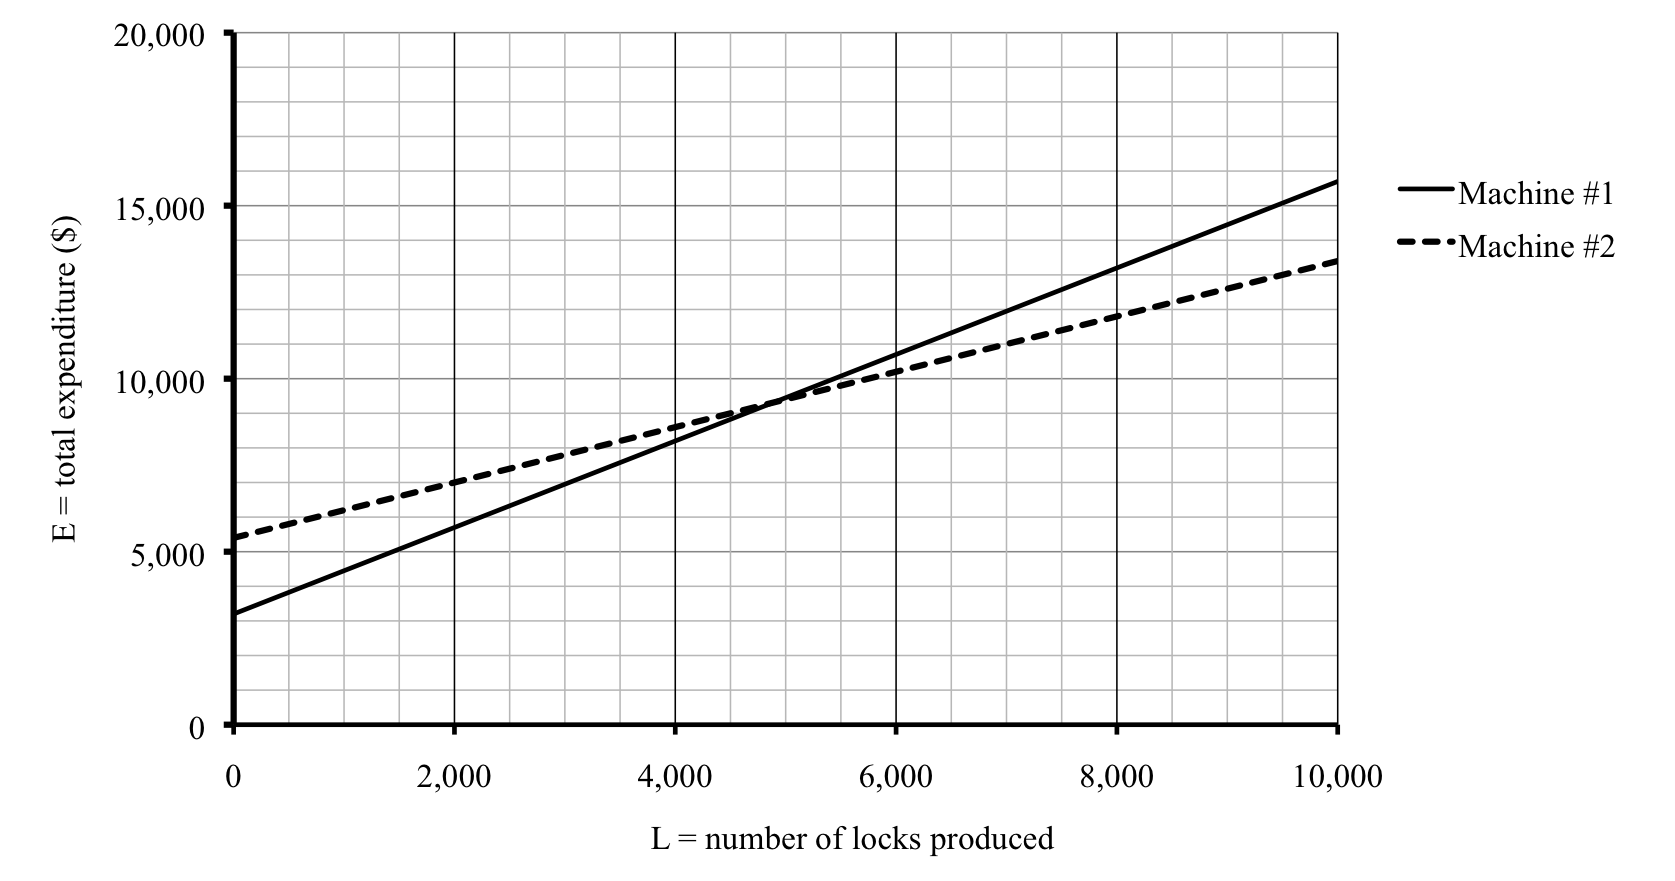
\includegraphics [width = 6in] {locks.png}}
\end{center}

A quick successive approximation narrows down the answer.
\begin{center}
\begin{tabular} {|c| |c |c |c |c |c |c |c |c|}\hline
$L$ & \text{4,000} & \text{6,000}& \text{5,000} & \text{4,500} & \text{4,800} & \text{4,900} \\ \hline
$E$ (for Machine \#1)   & \text{8,200} & \text{10,700} & \text{9,450} & \text{8,825} & \text{9,200} & \text{9,325} \\ \hline
$E$ (for Machine \#2) &  \text{8,600} & \text{10,200} & \text{9,400} & \text{9,000} & \text{9,240}& \text{9,320} \\ \hline
Less expensive option & \#1 & \#2 & \#2 & \#1 & \#1 & \#2 \\ \hline
\end{tabular}
\end{center}
So the choice changes somewhere between \text{4,800} and \text{4,900} locks.

There is a way for Quia Xun to solve the problem symbolically; we refer to this process as \textbf{solving the system}.  She wants to find the number of locks where 
$$\text{cost of Machine \#1} = \text{cost of Machine \#2}$$
Using her equations $E  =\text{3,200} + 1.25L$ for Machine \#1 and $E  =\text{5,400} + .80L$ for Machine \#2 she has
$$\text{3,200} + 1.25L=\text{5,400} + .80L$$
She wants to find the value of $L$ that makes both sides the same number.  To solve, Quia Xun subtracts \text{3,200}, the smaller of the two purchase prices, from each side to get
  \begin{eqnarray*}
\cancel{\text{3,200}} + 1.25L & = & \text{5,400} + .80L \\
-\cancel{\text{3,200}} \hspace{.5 in} & & -\text{3,200}  \\ %HSPACE
\end{eqnarray*}
\vspace{-.5in} %VSPACE

\noindent which simplifies to $$1.25L = \text{2,200} + .80L$$
Pause for a minute.  What does that \$\text{2,200} mean in the story?  It's the extra cost of buying Machine \#2 because $\$\text{5,400} - \$\text{3,200} = \$\text{2,200}$.  

What next?  This equation has the variable $L$ on each side.  Quia Xun needs to combine them somehow.  Here's how to do that.  Subtract $.80L$ from each side. Look closely.  She is subtracting $.80L$, not just $.80$.  We get
\begin{eqnarray*}
1.25L & = & \text{2,200} + \cancel{.80L}\\
-.80L & & \hspace{.4in}-\cancel{.80L}  \\ %HSPACE
\end{eqnarray*}
\vspace{-.5in} %VSPACE

\noindent How do we simplify $1.25L-.80L$?  Think about what these numbers represent in the story.  The cost was \$1.25 per lock versus \$.80 per lock.   The difference is \$1.25-\$.80 = \$.45 per lock.  So that means
$$1.25L -.80L = .45L$$ Think:  125 apples $-$ 80 apples $=$ 45 apples.  %Sily?
She can now simplify her equation to get
$$.45L = \text{2,200}$$
Ah, she can solve this equation just by dividing each side by .45 to get
$$\frac{\cancel{.45}L}{\cancel{.45}}= \frac{\text{2,200}}{.45}$$
which simplifies to $$L = \frac{\text{2,200}}{.45}= \text{2,200} \div .45 = 4888.88888\ldots \approx \text{4,889} \text{ locks}$$
If they plan to produce 4,889 locks or more, Quia Xun should go ahead and buy the more expensive machine, Machine \#2. Yeah, that's what we guessed -- just under \text{4,900} locks is the payoff.

She solved an equation here, but Quia Xun really wanted to know when $$\text{Machine \#1} \ge \text{Machine \#2}$$
so she could have solved the inequality $$\text{3,200} + 1.25L \ge \text{5,400} + 0.80L$$
instead.  
Check that the same steps give 
$$L \ge 4,889 \text{ locks}$$

 %\section{Systems of linear equations}

\begin{center}
\line(1,0){300} %\line(1,0){250}
\end{center}

\section*{Homework}

\noindent \textbf{Start by doing Practice exercises \#1-4 in the workbook.}

\bigskip

\noindent \textbf{Do you know \ldots}

\begin{itemize} 
\item How to compare two linear functions using a table? 
\item How to graph two linear functions on the same axes? 
\item What the solution of a linear system means in terms of the story? 
\item Where to look on a graph to see the solution of a linear system? 
\item How to successively approximate the solution of a linear system? 
\item How to solve a linear system? 
\item When to use inequality instead of an equation for a linear system? 
 \item[~] \textbf{If you're not sure, work the rest of exercises and then return to these questions.  Or, ask your instructor or a classmate for help.}  
\end{itemize}

\subsection*{Exercises}

\begin{enumerate} 
\setcounter{enumi}{4}

\item Just when Quia Xun thought she had things figured out, another possible option emerged.  She can outsource her lock production to a different plant at the cost of  \$1.55 per lock.   While that's more expensive per lock, it avoids having to buy a machine at all.  Recall her first two options were
\begin{center}
\begin{tabular} {ll}
$$\textbf{Machine \#1:} & E  =3,200 + 1.25L$$ \\
$$\textbf{Machine \#2:} & E  =5,400 + 0.80L$$ \\ 
\end{tabular}
\end{center}
where $E$ is the total expenditure to produce $L$ locks on that machine.  
\begin{enumerate}
\item  Write an equation showing how $E$ depends on $L$ if Quia Xun decides to outsource lock production.
\item For what number of locks does outsourcing make financial sense versus Machine \#1?  Set up and solve a system of equations.
\item Repeat for Machine \#2.
\end{enumerate}  

\item Don't ask why I know this, but it takes me 80 seconds per square foot to wash a floor using a rag.  If I use a mop, it's slightly quicker at 75 seconds per square foot, but another 3 minutes at the end to wring out the mop.  (The rag just pops in the washing machine.)
\begin{enumerate}
\item Name the variables and write an equation for each option: rag versus mop.  

\emph{Hint:  time is the dependent variable}
\item Set up and solve the system to determine the area of a room where either option takes the same amount of total time.
\item What do you suggest for each room?  (Note: find the area by multiplying the length times the width.)  My bathroom floor is 5'$\times$5'.   My kitchen floor is 8'$\times$10'.  The laundry room is 10'$\times$14'.
\end{enumerate}

\item Maria needed to replace the light bulb in the hallway.  When she went to the home improvement store she was overwhelmed with the choices of light bulbs.  One option is a compact fluorescent light  (CFL) bulb.  A CFL bulb costs \$1.  This fixture will cost \$0.95 per month to run with a CFL bulb.  A different option Maria is considering is a light-emitting diode (LED) instead of a bulb.  A LED costs \$24 but reduces the cost for the fixture to  \$0.60 per month.    
\begin{enumerate}
\item Name the variables and write an equation for each option: LED versus CFL.
\item Compare the total cost for each bulb for 1, 6, 18, and 36 months.
\item Draw a graph showing both functions on the same axes.
\item Set up and solve a system of linear equations to determine the payback time.
\item Based on what you've learned, fill in the blank and circle the correct word.
\begin{quote}
The more expensive LED pays off if Maria is going to use it for \underline{\quad~}  or more months.  
\end{quote}
\end{enumerate}

\item The community center offers exercise classes on a pay-as-you-go basis.  It normally costs \$20 to register and then \$15 per exercise class.  Alternatively, you can pay \$150 to become a member, and then \$10 per exercise class.  If we let $E$ represent the number of exercise classes I attend and $T$ represent the total cost in dollars, then the equations are:
\begin{center}
\begin{tabular} {ll}
\textbf{Pay as-you-go:} & $T = 20 + 15E$ \\
\textbf{Member:} & $T= 150 + 10E$ \\ 
\end{tabular}
\end{center}  
\begin{enumerate}
\item Create a table of reasonable values and draw a graph showing both options.
\item According to your graph, what is the break even point?  
\item Use successive approximations to find the break even point.
\item Set up and solve a system of linear equations to determine the exact break even point
\item Describe in words what you've learned about whether or not to buy membership.
\end{enumerate}

\item The weekly supply $S$ and demand $D$ for corn-on-the-cob (in hundreds) at a local market are given by the equations 
\begin{center}
\begin{tabular} {ll}
\textbf{Supply:} & $S = 1.5P+6$ \\
\textbf{Demand:} & $D= 11 - 0.9P$ \\ 
\end{tabular}
\end{center} 
where $P$ is the price per unit, in dollars per dozen.
\begin{enumerate}
\item Is there a shortage or surplus if corn is priced at \$3.25/dozen?  What if it's priced at \$1.75/dozen?
\item Set up and solve an equation to find the equilibrium price of corn.
\item Make a small table of values and graph.  Does your answer to (b) agree with your graph?  Explain.
\end{enumerate}

\item A solar heating system costs approximately \$30,000 to install and \$150 per year to run.  By comparison, a gas heating system costs approximately \$12,000 to install and \$700 per year to run.   Earlier we wrote equations showing how the total cost \$$T$ depends on the time, $Y$ years.
\begin{center}
\begin{tabular} {ll}
\textbf{Solar:} & $T  =30,000 + 150Y$\\
\textbf{Gas:} & $T  = 12,000 + 700Y$ \\ 
\end{tabular}
\end{center}

\hfill \emph{Story also appears in 4.1 \#1}
\begin{enumerate}
\item Set up an solve a system to determine the payback time of installing the solar heating system.
\item How does the payback time change if the state offers a \$7,000 rebate?  That means, in effect, that the solar system costs \$7,000 less to install. Write a new equation for the solar heating system.  Then set up and solve the new system.
\item How high a rebate would the state have to offer to insure a payback time of 15 years?  \emph{Hint:  compare the costs of gas and solar heating systems at 15 years.}
\end{enumerate}

\end{enumerate}
